\section{Manual de Usuario}

\begin{enumerate}
\def\labelenumi{\arabic{enumi}.}
\item
  Para poder utilizar el vehículo, se debe tener la aplicación BLE
  Joystick instalada en un teléfono Android.
  
\url{https://play.google.com/store/apps/details?id=iyok.com.blejoystick}
\item
  El vehículo contiene una llave para cortar la alimentación de
  baterías:
\end{enumerate}

\begin{figure}[H]
\centering
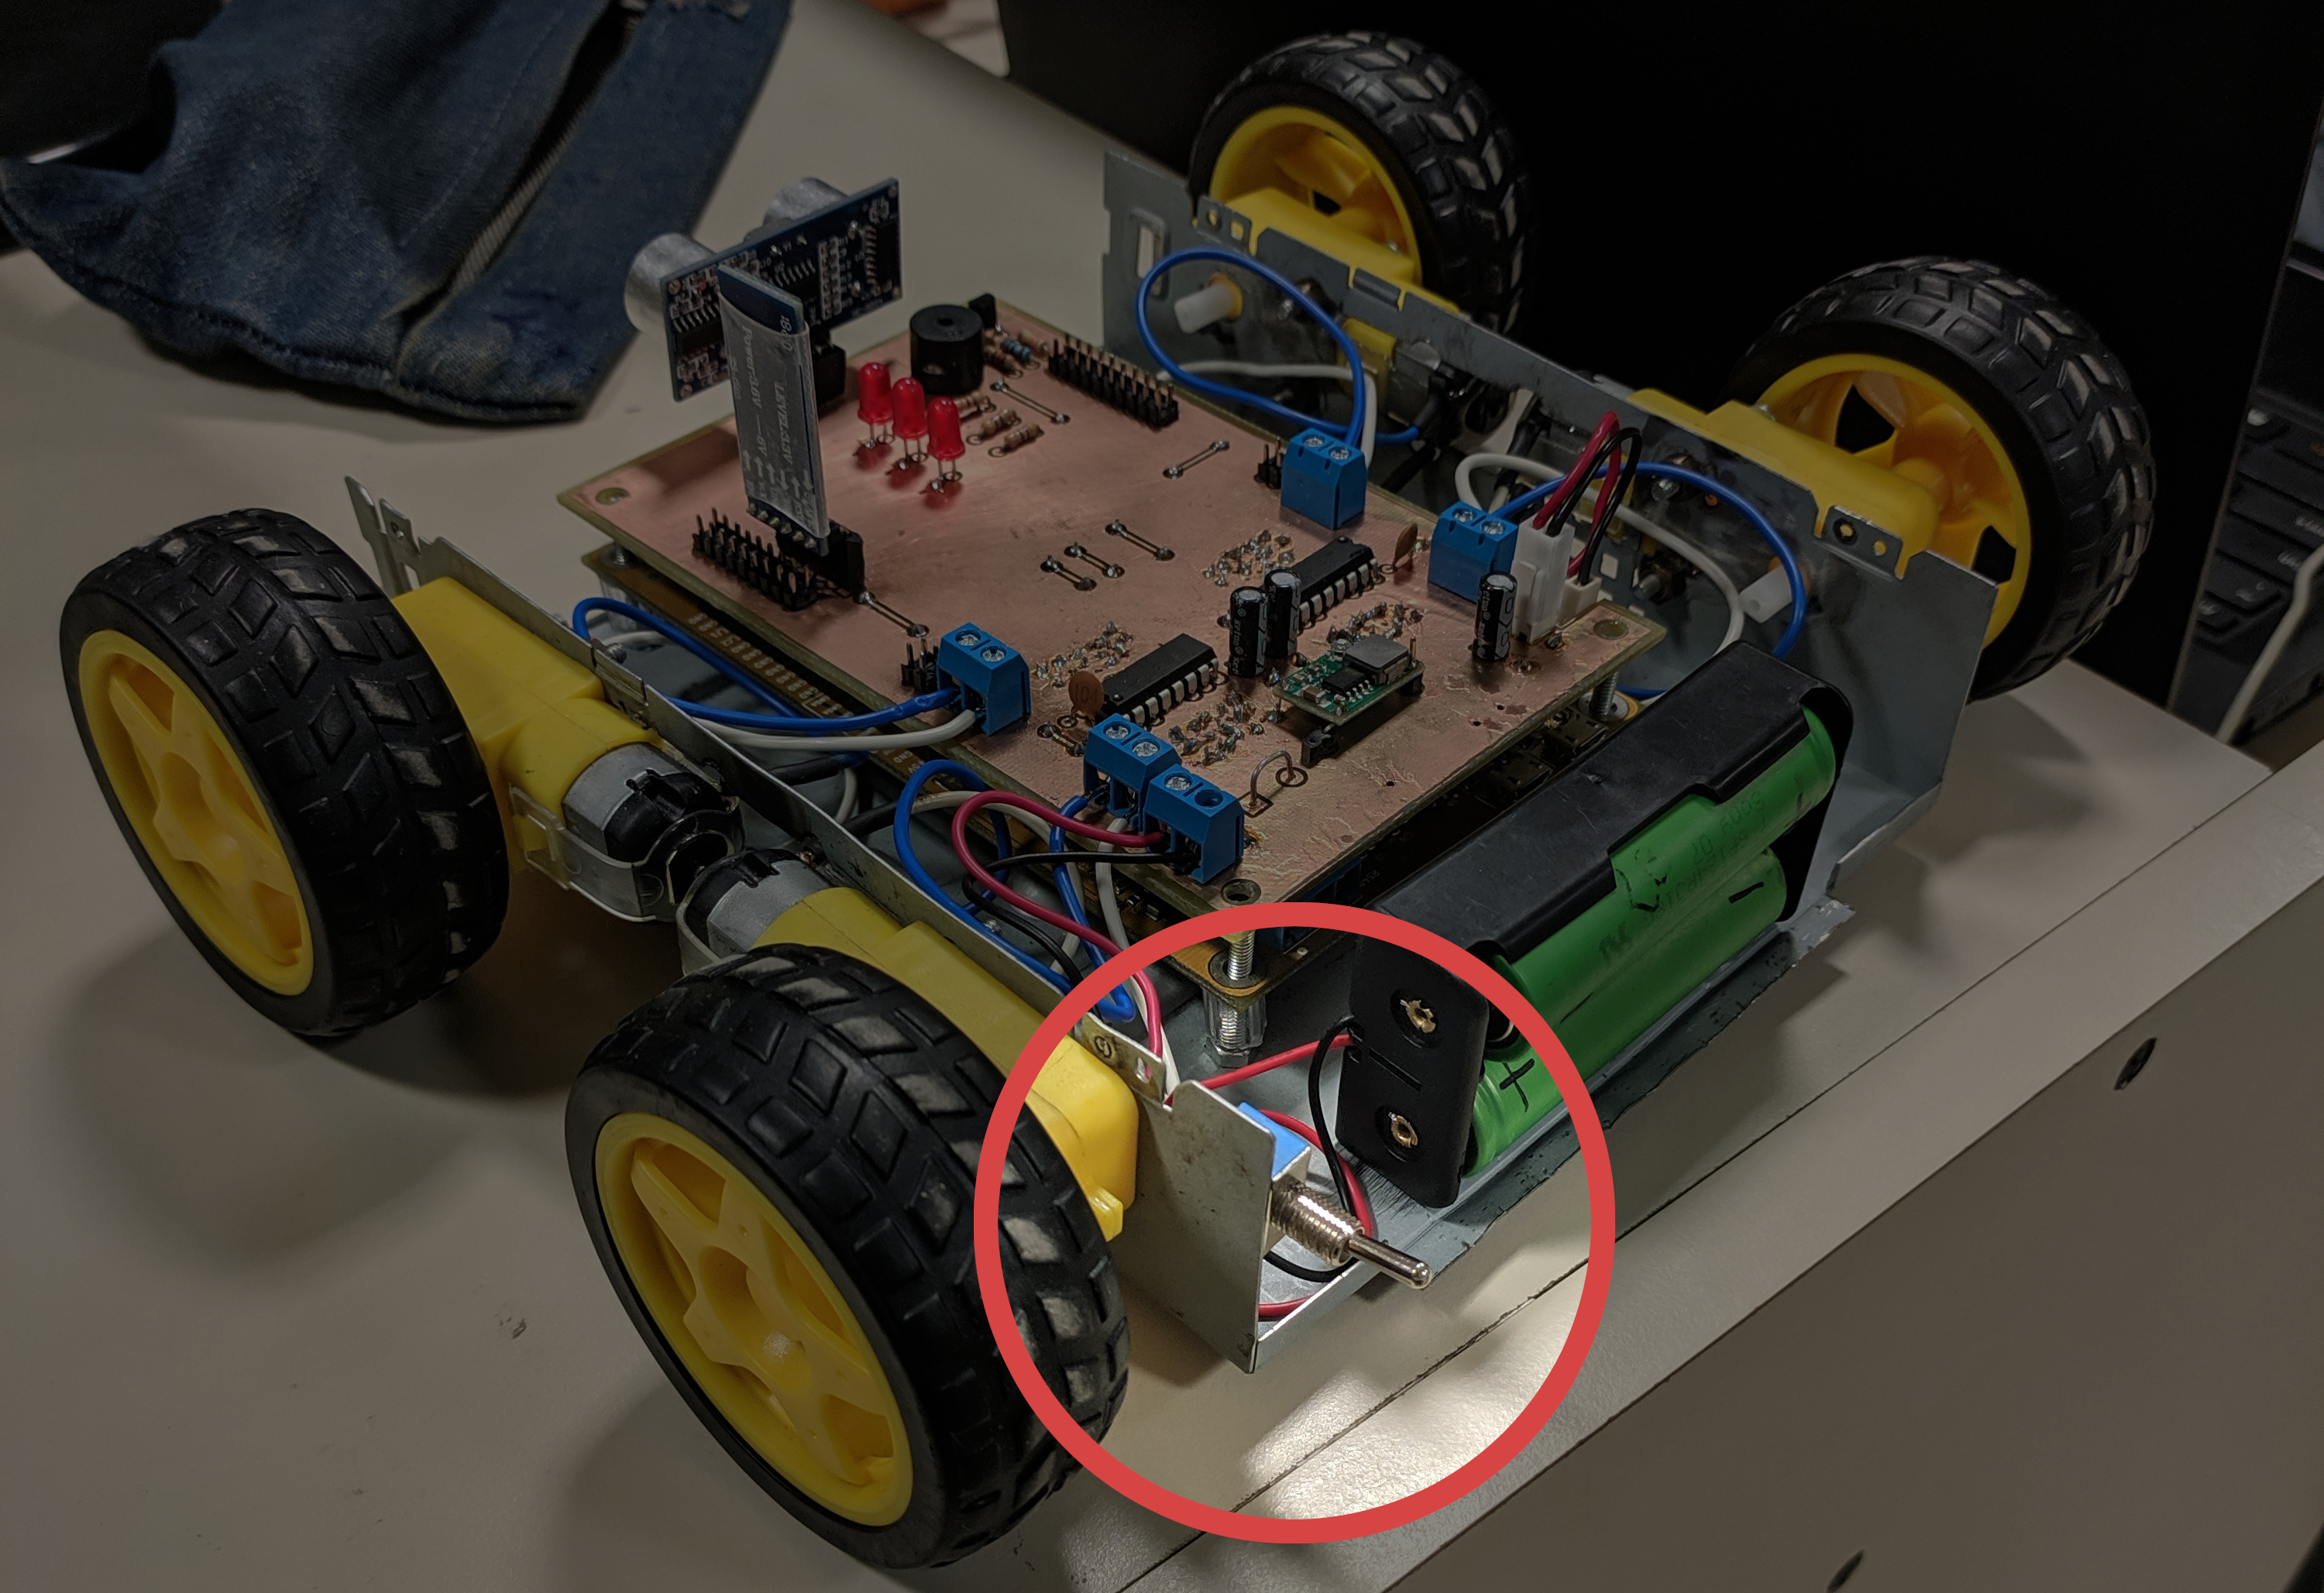
\includegraphics[width=0.8\linewidth]{informe_4/llave.jpg}
\caption{Llave de encendido}
\end{figure}

\begin{enumerate}
\def\labelenumi{\arabic{enumi}.}
\setcounter{enumi}{2}
\tightlist
\item
Conectar el teléfono al módulo Bluetooth del vehículo, una vez establecida la conexión, el LED del módulo HM-10 quedará fijo y dejará de titilar.
\end{enumerate}
